\documentclass[11pt]{article}
\usepackage[T1]{fontenc}
\usepackage{lmodern}
\usepackage{microtype}
\DisableLigatures[f]{encoding = *, family = *}
\usepackage[margin=1.15in]{geometry}
\usepackage{setspace}
\usepackage{booktabs}
\usepackage{float}
\usepackage{amsmath}
\usepackage{pgfplots}
\pgfplotsset{compat=1.16}
\usepgfplotslibrary{fillbetween}
\usepackage{fancyhdr}
\pagestyle{fancy}
\fancyhf{}
\fancyhead[C]{\small SYNTHETIC TEST PAPER, NOT REAL RESEARCH}
\fancyfoot[C]{\thepage}
\renewcommand{\headrulewidth}{0pt}
\setstretch{1.3}
\newcommand{\tn}[1]{\par\vspace{2pt}{\footnotesize #1}}

\title{Slack, Rivals, and Exploration: Curvilinear and Contingent Effects in a Panel of Mid-Sized Manufacturers}
\author{Marta Voskuijlen\\ Halverson School of Management (fictional)}
\date{}

\begin{document}
\maketitle
\thispagestyle{fancy}
\begin{center}
{\bfseries SYNTHETIC TEST PAPER, NOT REAL RESEARCH}\\[4pt]
{\small All firms, people, institutions, data, and results in this paper are invented for testing a review tool. The reference list names real methods papers only as background.}
\end{center}

\begin{abstract}
\noindent Organizational slack is said to help exploration up to a point and to hurt it beyond that point. Using a fictional panel of 412 mid-sized manufacturers observed from 2004 to 2019, we estimate an inverted-U relationship between slack and exploratory patenting, and we ask how CEO tenure, the number of rival firms, analyst coverage, family ownership, and alliance experience change that relationship. We also study alliance formation and market entry with logit models. Slack has an inverted-U relationship with exploratory patenting, tenure steepens it, and rivals weaken the pull of research and development, most of all when analyst coverage is high. We discuss what the results imply for the design of slack policies.
\end{abstract}

\section{Introduction}

Managers and scholars have long held that resources beyond current needs can be put to good or bad use. A cushion of slack gives a firm room to experiment, yet a large cushion removes the pressure to choose carefully. This tension has been written as a curvilinear hypothesis: exploration rises with slack, peaks, and then falls (Pierce and Aguinis 2013; Haans et al. 2016). We test that hypothesis in a panel of mid-sized manufacturers, and we extend it to the conditions under which the curve changes.

We make three contributions. First, we document an inverted-U relationship between slack and exploratory patenting in a setting where slack is measured at the firm-year level and exploration is measured by patents in technology classes that are new to the firm. Second, we show that the curve depends on the tenure of the chief executive. Third, we show that the influence of research and development on exploration depends on the number of rivals and on the amount of attention that analysts pay to the firm.

The paper proceeds as follows. Section 2 develops seven hypotheses. Section 3 describes the data and methods. Section 4 reports the results, Section 5 reports additional analyses, and Section 6 discusses the findings.

\section{Theory and Hypotheses}

\paragraph{Slack and exploration.} Slack provides the funds and the tolerance for failure that exploration needs. At low levels, added slack loosens constraints and allows managers to fund projects outside the firm's current technology base. At high levels, added slack weakens discipline and directs resources to projects that would not survive scrutiny. We therefore expect exploration to first rise and then fall.

\emph{Hypothesis 1 (H1).} Organizational slack has an inverted-U relationship with exploratory patenting.

\paragraph{CEO tenure.} Long-tenured chief executives hold more discretion and more attachment to the existing business. Where discretion is high, the same amount of slack has a sharper effect on the resources that reach exploratory projects, and the penalty for excess is also sharper.

\emph{Hypothesis 2 (H2).} CEO tenure steepens the inverted-U relationship between slack and exploratory patenting.

\paragraph{Rivals and research spending.} Firms that spend more on research and development tend to explore more. The number of direct rivals changes how much of that spending is directed to new technology classes, because rivals raise the cost of staying with a shared technology.

\emph{Hypothesis 3 (H3).} The number of rivals moderates the relationship between research and development intensity and exploratory patenting.

\paragraph{Family ownership.} Family owners tend to hold long horizons and to protect the firm from forced short-term choices. Slack should therefore convert into exploration more readily where families own the firm.

\emph{Hypothesis 4 (H4).} The relationship between slack and exploratory patenting is stronger for family firms than for nonfamily firms, and it is stronger in the later part of the sample.

\paragraph{Alliances.} Research and development spending raises the odds that a firm finds a partner, but firms that have formed many alliances rely less on new research to find partners.

\emph{Hypothesis 5 (H5).} Alliance experience weakens the effect of research and development intensity on the probability of forming an alliance.

\paragraph{Attention.} Analysts direct attention toward firms and away from others, and their attention raises the visibility of rivalry.

\emph{Hypothesis 6 (H6).} The moderating effect of the number of rivals on the relationship between research and development intensity and exploration is stronger when analyst coverage is high.

\paragraph{Market entry.} Slack lets firms enter new markets, and favorable market conditions make entry more attractive.

\emph{Hypothesis 7 (H7).} Market munificence strengthens the effect of slack on the probability of entering a new market.

\section{Data and Methods}

\subsection{Sample}

The sample is an unbalanced firm-year panel of 412 fictional mid-sized manufacturers observed from 2004 to 2019, which gives 3,296 firm-years. Of the 412 firms, 128 are family firms. Table~\ref{tab:desc} reports descriptive statistics.

\subsection{Measures}

\paragraph{Dependent variables.} Exploratory patenting is the count of patents granted in technology classes in which the firm held no patent in the previous five years. Because the count has a long right tail, our dependent variable in the linear models is the natural logarithm of one plus the count of exploratory patents. Alliance formation equals one if the firm formed at least one alliance in the year, and market entry equals one if the firm entered a new product market in the year.

\paragraph{Independent variables.} Slack is the ratio of liquid assets to operating costs, and it ranges from 0 to 3.10 in the sample. Team size is the number of members of the top management team and CEO tenure is the number of years the chief executive has held the post; neither is centered. Research and development intensity is research and development spending over sales, standardized. Rivals is the number of direct rivals in the firm's main product market, and analyst coverage is the number of analysts who cover the firm. Supplier concentration is the share of purchases from the largest supplier; we center it at its mean of 0.40 before squaring it. Market munificence is the growth of industry sales. Alliance experience is the count of alliances formed in earlier years, and prior alliance equals one if any alliance was formed in the previous three years.

\begin{table}[H]
\centering
\caption{Descriptive statistics}\label{tab:desc}
{\small
\begin{tabular}{lrrrr}
\toprule
Variable & Mean & SD & Min & Max \\
\midrule
Exploratory patents (count) & 2.90 & 6.80 & 0 & 61 \\
Log(1 + exploratory patents) & 0.68 & 1.05 & 0 & 4.13 \\
Slack & 1.02 & 0.74 & 0 & 3.10 \\
Team size & 8.1 & 2.9 & 3 & 15 \\
CEO tenure (years) & 8.4 & 5.2 & 1 & 22 \\
R\&D intensity (standardized) & 0.00 & 1.00 & $-1.48$ & 4.26 \\
Rivals & 5.2 & 1.8 & 2 & 9 \\
Analyst coverage & 1.5 & 2.4 & 0 & 14 \\
Supplier concentration & 0.40 & 0.21 & 0.02 & 0.98 \\
Alliance formation (0/1) & 0.40 & 0.49 & 0 & 1 \\
Market entry (0/1) & 0.18 & 0.38 & 0 & 1 \\
Family firm (0/1) & 0.31 & 0.46 & 0 & 1 \\
Alliance experience & 1.9 & 2.2 & 0 & 11 \\
Prior alliance (0/1) & 0.52 & 0.50 & 0 & 1 \\
Market munificence & 0.11 & 0.92 & $-2.40$ & 2.90 \\
Firm size (log assets) & 5.9 & 1.1 & 3.2 & 9.4 \\
Leverage & 0.24 & 0.15 & 0.00 & 0.91 \\
\bottomrule
\end{tabular}}
\tn{Notes: 3,296 firm-years from 412 firms. Fifty-eight percent of firm-years have zero exploratory patents.}
\end{table}

\subsection{Estimation}

The linear models include firm and year fixed effects, and standard errors are clustered by firm. The logit models in Table~\ref{tab:logit} include industry and year fixed effects rather than firm effects, because many firms never change status and would drop from a firm fixed-effects logit; standard errors are clustered by firm. Rivals, analyst coverage, and research and development intensity vary within firm and year, so their coefficients and interactions are identified in all models.

To reduce multicollinearity between a product term and its components, we mean-center slack and analyst coverage before forming their product in the robustness models of Appendix Table~\ref{tab:a2}. That table also reports the uncentered version.

\section{Results}

\subsection{Slack and exploration (H1)}

Column 1 of Table~\ref{tab:main} reports the test of H1. The coefficient on slack is 0.84 and the coefficient on slack squared is $-0.078$. Both are statistically significant, and the negative squared term is consistent with an inverted U. The turning point implied by the two coefficients is 5.38, which locates the peak of the curve. The turning point is therefore an optimal level of slack in the interior of the distribution, and we conclude that H1 is supported. Figure~\ref{fig:slack} plots the fitted curve. Because the outcome is the logarithm of one plus the patent count, the coefficient of 0.84 says that a one-unit increase in slack raises exploratory patenting by about 84 percent at low levels of slack.

\begin{table}[H]
\centering
\caption{Slack, CEO tenure, and exploratory patenting}\label{tab:main}
{\small
\begin{tabular}{lcc}
\toprule
 & (1) & (2) \\
Dependent variable: log(1 + exploratory patents) & H1 & H2 \\
\midrule
Slack & 0.84$^{***}$ & 0.87$^{***}$ \\
 & (0.21) & (0.22) \\
Slack squared & $-0.078^{**}$ & $-0.10^{***}$ \\
 & (0.031) & (0.033) \\
CEO tenure & & 0.021$^{*}$ \\
 & & (0.012) \\
Slack $\times$ CEO tenure & & 0.010$^{**}$ \\
 & & (0.004) \\
Slack squared $\times$ CEO tenure & & 0.008$^{***}$ \\
 & & (0.003) \\
Firm size & 0.31$^{***}$ & 0.30$^{***}$ \\
 & (0.09) & (0.09) \\
Leverage & $-0.42^{***}$ & $-0.40^{***}$ \\
 & (0.15) & (0.15) \\
\midrule
Firm and year fixed effects & Yes & Yes \\
Observations & 3,296 & 3,296 \\
Firms & 412 & 412 \\
Within R$^2$ & 0.21 & 0.24 \\
\bottomrule
\end{tabular}}
\tn{Notes: Standard errors clustered by firm in parentheses. $^{*}p<0.10$, $^{**}p<0.05$, $^{***}p<0.01$. Slack ranges from 0 to 3.10 and CEO tenure from 1 to 22 years, both uncentered.}
\end{table}

\begin{figure}[H]
\centering
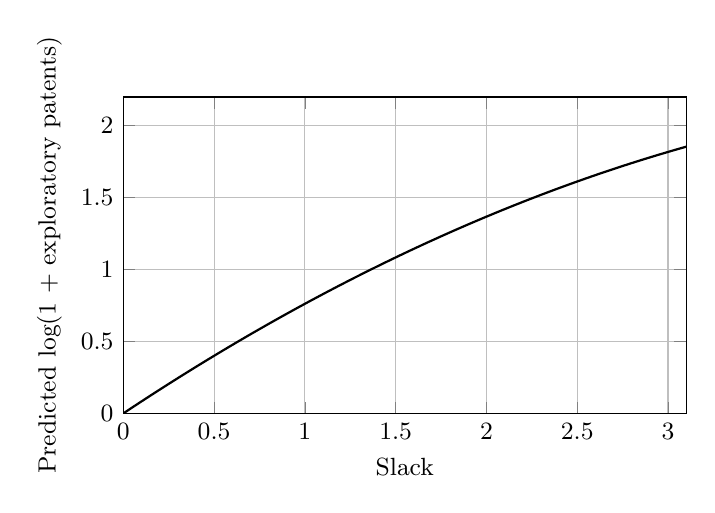
\begin{tikzpicture}
\begin{axis}[width=0.72\textwidth,height=5.6cm,xlabel={Slack},ylabel={Predicted log(1 + exploratory patents)},xmin=0,xmax=3.1,ymin=0,ymax=2.2,grid=major,every axis label/.append style={font=\small},tick label style={font=\small}]
\addplot[thick,domain=0:3.1,samples=40]{0.84*x-0.078*x^2};
\end{axis}
\end{tikzpicture}
\caption{Fitted relationship between slack and exploratory patenting, from column 1 of Table~\ref{tab:main}, over the observed range of slack.}\label{fig:slack}
\end{figure}

\subsection{CEO tenure (H2)}

Column 2 of Table~\ref{tab:main} adds CEO tenure and its interactions with slack and slack squared. The coefficient on slack times tenure is positive (0.010) and significant. We read this as evidence that CEO tenure steepens the inverted U, so H2 is supported. We do not plot the curve at low and high values of tenure because the sign of the interaction is clear.

\subsection{Rivals and research spending (H3)}

Column 1 of Table~\ref{tab:rivals} reports the model with research and development intensity, the number of rivals, and their product. The effect of R\&D intensity on exploration is positive (b = 0.31) and significant, and the negative product term shows that rivals weaken it. H3 is supported.

\begin{table}[H]
\centering
\caption{Research spending, rivals, and analyst coverage}\label{tab:rivals}
{\small
\begin{tabular}{lcc}
\toprule
 & (1) & (2) \\
Dependent variable: log(1 + exploratory patents) & H3 & H6 \\
\midrule
R\&D intensity & 0.31$^{***}$ & 0.29$^{**}$ \\
 & (0.11) & (0.12) \\
Rivals & $-0.048$ & $-0.041$ \\
 & (0.031) & (0.029) \\
Analyst coverage & & 0.012 \\
 & & (0.010) \\
R\&D intensity $\times$ rivals & $-0.020^{**}$ & $-0.018^{**}$ \\
 & (0.008) & (0.008) \\
R\&D intensity $\times$ analyst coverage & & 0.061$^{***}$ \\
 & & (0.021) \\
R\&D intensity $\times$ rivals $\times$ analyst coverage & & $-0.006^{***}$ \\
 & & (0.002) \\
Rivals $\times$ analyst coverage & & Not included \\
\midrule
Controls, firm and year fixed effects & Yes & Yes \\
Observations & 3,296 & 3,296 \\
Within R$^2$ & 0.22 & 0.25 \\
\bottomrule
\end{tabular}}
\tn{Notes: Standard errors clustered by firm in parentheses. $^{*}p<0.10$, $^{**}p<0.05$, $^{***}p<0.01$. Rivals ranges from 2 to 9. Controls are firm size and leverage.}
\end{table}

\subsection{Analyst coverage as a moderator}

Column 2 of Table~\ref{tab:rivals} also lets analyst coverage moderate the effect of research and development intensity. Figure~\ref{fig:coverage} plots the predicted relationship between R\&D intensity and exploration at low and high analyst coverage, holding rivals at its mean. Low coverage is defined as the mean minus one standard deviation and high coverage as the mean plus one standard deviation. The slope is steeper at high coverage, which agrees with the positive product term.

\begin{figure}[H]
\centering
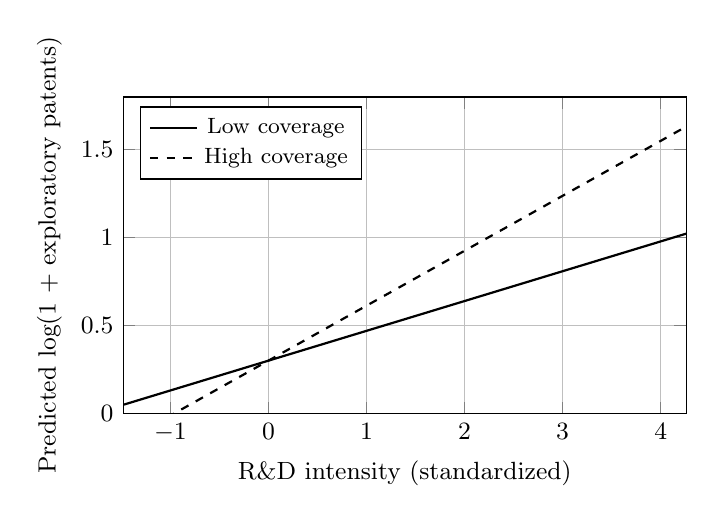
\begin{tikzpicture}
\begin{axis}[width=0.72\textwidth,height=5.6cm,xlabel={R\&D intensity (standardized)},ylabel={Predicted log(1 + exploratory patents)},xmin=-1.48,xmax=4.26,ymin=0,ymax=1.8,grid=major,legend pos=north west,legend style={font=\footnotesize},every axis label/.append style={font=\small},tick label style={font=\small}]
\addplot[thick,domain=-1.48:4.26,samples=2]{0.3+0.1696*x};
\addlegendentry{Low coverage}
\addplot[thick,dashed,domain=-1.48:4.26,samples=2]{0.3+0.3126*x};
\addlegendentry{High coverage}
\end{axis}
\end{tikzpicture}
\caption{Predicted exploratory patenting by R\&D intensity at low (mean minus 1 SD) and high (mean plus 1 SD) analyst coverage, from column 2 of Table~\ref{tab:rivals}.}\label{fig:coverage}
\end{figure}

\subsection{Family ownership and time (H4)}

Table~\ref{tab:family} reports the slack relationship in separate samples of family and nonfamily firms, using a specification that is linear in slack. The coefficient is 0.70 for family firms and 0.40 for nonfamily firms. The coefficient is statistically significant for family firms and is not for nonfamily firms. The slack effect exists only for family firms, and H4 is supported for ownership.

\begin{table}[H]
\centering
\caption{Slack and exploratory patenting by family ownership and period}\label{tab:family}
{\small
\begin{tabular}{lccc}
\toprule
 & \multicolumn{2}{c}{Panel A: separate samples} & Panel B: pooled \\
 & Family firms & Nonfamily firms & All firms \\
\midrule
Slack & 0.70$^{***}$ & 0.40 & 0.50$^{***}$ \\
 & (0.26) & (0.26) & (0.18) \\
Slack $\times$ post-2012 & & & 0.14$^{***}$ \\
 & & & (0.05) \\
\midrule
Controls, firm and year fixed effects & Yes & Yes & Yes \\
Observations & 1,025 & 2,271 & 3,296 \\
Firms & 128 & 284 & 412 \\
\bottomrule
\end{tabular}}
\tn{Notes: Dependent variable is log(1 + exploratory patents). Standard errors clustered by firm in parentheses. $^{*}p<0.10$, $^{**}p<0.05$, $^{***}p<0.01$. Year fixed effects absorb the post-2012 main effect.}
\end{table}

\subsection{The later part of the sample (H4 continued)}

Panel B of Table~\ref{tab:family} pools all firms and adds the interaction of slack with an indicator for the years after 2012. The interaction is 0.14 and significant, so the slack effect is stronger after 2012. This supports the second part of H4.

\subsection{Alliance formation (H5)}

Column 1 of Table~\ref{tab:logit} reports a logit model of alliance formation. The interaction between research and development intensity and alliance experience is negative ($-0.21$) and significant. Alliance experience weakens the effect of R\&D on the probability of forming an alliance, so H5 is supported. An odds ratio of 1.8 on prior alliance means firms with a prior alliance are 80 percent more likely to form one.

\begin{table}[H]
\centering
\caption{Logit models of alliance formation and market entry}\label{tab:logit}
{\small
\begin{tabular}{lcc}
\toprule
 & (1) & (2) \\
 & Alliance formation & Market entry \\
 & H5 & H7 \\
\midrule
R\&D intensity & 0.35$^{***}$ & \\
 & (0.11) & \\
Alliance experience & 0.18$^{**}$ & \\
 & (0.08) & \\
R\&D intensity $\times$ alliance experience & $-0.21^{***}$ & \\
 & (0.08) & \\
Prior alliance & 0.59$^{***}$ & \\
 & (0.14) & \\
Slack & & 0.22$^{**}$ \\
 & & (0.10) \\
Market munificence & & 0.15 \\
 & & (0.11) \\
Slack $\times$ market munificence & & 0.19$^{***}$ \\
 & & (0.07) \\
Firm size & 0.27$^{***}$ & 0.24$^{***}$ \\
 & (0.07) & (0.07) \\
\midrule
Industry and year fixed effects & Yes & Yes \\
Observations & 3,296 & 3,296 \\
\bottomrule
\end{tabular}}
\tn{Notes: Log-odds coefficients; standard errors clustered by firm in parentheses. $^{*}p<0.10$, $^{**}p<0.05$, $^{***}p<0.01$. The base rate of alliance formation is 0.40 (Table~\ref{tab:desc}).}
\end{table}

\subsection{Rivals and analyst coverage (H6)}

The three-way interaction in column 2 of Table~\ref{tab:rivals} is negative ($-0.006$) and significant. The moderating effect of rivals is strongest when analyst coverage is high, so H6 is supported. Rivals and analyst coverage each vary within firm and year, so their own terms are identified in this model.

\clearpage
\subsection{Market entry (H7)}

Column 2 of Table~\ref{tab:logit} reports a logit model of market entry. H7 concerns the probability of entry, so we evaluate the interaction on the probability scale. The average second difference in the probability of entry, moving slack and market munificence together from their 25th to their 75th percentiles, is 0.031 (95 percent confidence interval 0.012 to 0.050). The second difference has four cells: it is the change in the predicted probability of entry from the 25th to the 75th percentile of slack at the 75th percentile of munificence, minus the same change at the 25th percentile of munificence, averaged over firm-years. Figure~\ref{fig:entry} plots the predicted probability of entry against slack at low and high munificence with 95 percent confidence intervals. The effect of slack on entry is larger where munificence is high, and H7 is supported.

\begin{figure}[H]
\centering
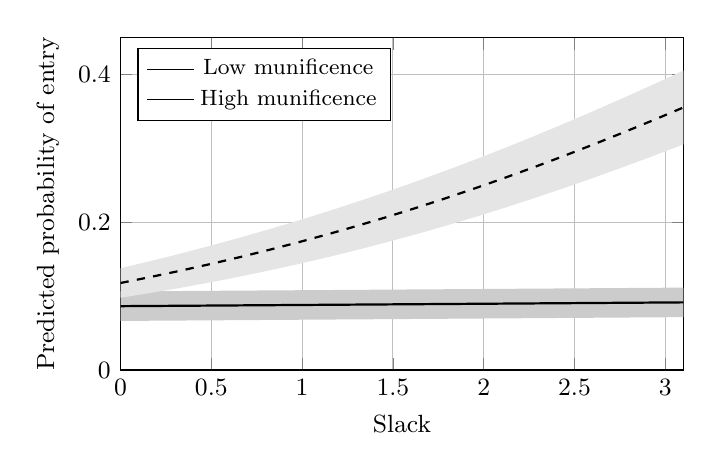
\begin{tikzpicture}
\begin{axis}[width=0.72\textwidth,height=5.8cm,xlabel={Slack},ylabel={Predicted probability of entry},xmin=0,xmax=3.1,ymin=0,ymax=0.45,grid=major,legend pos=north west,legend style={font=\footnotesize},every axis label/.append style={font=\small},tick label style={font=\small}]
\addplot[name path=lo1,draw=none,domain=0:3.1,samples=20]{(1/(1+exp(-(-2.2+0.15*(-1.05)+(0.22+0.19*(-1.05))*x))))-0.02};
\addplot[name path=hi1,draw=none,domain=0:3.1,samples=20]{(1/(1+exp(-(-2.2+0.15*(-1.05)+(0.22+0.19*(-1.05))*x))))+0.02};
\addplot[gray!40] fill between[of=lo1 and hi1];
\addplot[thick,domain=0:3.1,samples=20]{(1/(1+exp(-(-2.2+0.15*(-1.05)+(0.22+0.19*(-1.05))*x))))};
\addlegendentry{Low munificence}
\addplot[name path=lo2,draw=none,domain=0:3.1,samples=20]{(1/(1+exp(-(-2.2+0.15*1.25+(0.22+0.19*1.25)*x))))-0.02-0.03*x/3.1};
\addplot[name path=hi2,draw=none,domain=0:3.1,samples=20]{(1/(1+exp(-(-2.2+0.15*1.25+(0.22+0.19*1.25)*x))))+0.02+0.03*x/3.1};
\addplot[gray!20] fill between[of=lo2 and hi2];
\addplot[thick,dashed,domain=0:3.1,samples=20]{(1/(1+exp(-(-2.2+0.15*1.25+(0.22+0.19*1.25)*x))))};
\addlegendentry{High munificence}
\end{axis}
\end{tikzpicture}
\caption{Predicted probability of market entry by slack at low and high market munificence (the 10th and 90th percentiles, $-1.05$ and 1.25), with 95 percent confidence intervals, from column 2 of Table~\ref{tab:logit}.}\label{fig:entry}
\end{figure}

\section{Additional Analyses}

\subsection{Team size}

Column 1 of Table~\ref{tab:extra} adds a curvilinear term for team size, which ranges from 3 to 15 members and is not centered. The coefficient on team size is 0.12 and the coefficient on its square is $-0.0060$. The implied turning point is 10 members. Exploration declines beyond ten members. The covariance between the two coefficient estimates is not reported.

\clearpage
\subsection{Supplier concentration}

Column 2 of Table~\ref{tab:extra} adds a curvilinear term for supplier concentration. The raw variable ranges from 0.02 to 0.98 with a mean of 0.40, and we center it at the mean before squaring, so the centered variable ranges from $-0.38$ to 0.58. The coefficients are $-0.24$ for the linear term and $-1.20$ for the squared term, and the covariance between them is 0.006. The turning point is $-0.10$ on the centered scale, or 0.30 on the raw scale, and its 95 percent Fieller interval runs from $-0.22$ to $-0.02$ on the centered scale, which is inside the observed range. The slope is 0.67 at the lowest observed value and $-1.63$ at the highest, and each is distinguishable from zero at the 5 percent level.

\begin{table}[H]
\centering
\caption{Team size and supplier concentration}\label{tab:extra}
{\small
\begin{tabular}{lcc}
\toprule
Dependent variable: log(1 + exploratory patents) & (1) & (2) \\
\midrule
Team size & 0.12$^{***}$ & \\
 & (0.020) & \\
Team size squared & $-0.0060^{**}$ & \\
 & (0.0024) & \\
Supplier concentration (centered) & & $-0.24^{**}$ \\
 & & (0.10) \\
Supplier concentration (centered) squared & & $-1.20^{***}$ \\
 & & (0.30) \\
\midrule
Controls, firm and year fixed effects & Yes & Yes \\
Observations & 3,296 & 3,296 \\
\bottomrule
\end{tabular}}
\tn{Notes: Standard errors clustered by firm in parentheses. $^{*}p<0.10$, $^{**}p<0.05$, $^{***}p<0.01$. Team size is uncentered. The covariance of the two supplier concentration terms is 0.006.}
\end{table}

\clearpage
\subsection{Alliance counts}

To check the alliance results on a count scale, we estimate the number of alliances formed in a year with Poisson pseudo-maximum likelihood and firm fixed effects. Firms with no alliances in any year drop out of this model. Table~\ref{tab:count} reports the result. The incidence rate ratio of 1.12 means a 12 percent higher expected number of alliances for a one standard deviation increase in R\&D intensity.

\begin{table}[H]
\centering
\caption{Poisson model of the alliance count}\label{tab:count}
{\small
\begin{tabular}{lc}
\toprule
Dependent variable: alliances formed & (1) \\
\midrule
R\&D intensity & 0.113$^{***}$ \\
 & (0.041) \\
Incidence rate ratio & 1.12 \\
\midrule
Controls, firm and year fixed effects & Yes \\
Observations & 2,884 \\
Firms & 361 \\
\bottomrule
\end{tabular}}
\tn{Notes: Poisson pseudo-maximum likelihood; standard errors clustered by firm in parentheses. $^{***}p<0.01$.}
\end{table}

\section{Discussion}

We find that slack, tenure, rivals, and analyst attention shape how mid-sized manufacturers direct their resources to new technologies. The results speak to the design of slack policies. Our estimates identify the optimal slack level for a given firm, and a firm that wants to maximize its exploratory patenting can use the turning point as a target. Firms far below that level gain from adding slack, and the opposite holds for firms above it.

The findings on tenure suggest that boards should attend to the tenure of the chief executive when setting slack targets. The findings on rivals and analysts suggest that the value of research spending for exploration depends on the competitive and informational setting. The findings on alliances and entry suggest that experience and market conditions change what research and slack buy.

The study has limits. The panel is limited to mid-sized manufacturers, and we do not model the selection of firms into family ownership. We leave these questions for future work.

\section{Conclusion}

Slack, tenure, rivalry, and attention shape exploration in the panel we study. We hope the framework helps future work on how organizations turn resources into new technology.

\section*{References}
{\setstretch{1.1}\small\setlength{\parindent}{-1.5em}\setlength{\leftskip}{1.5em}
\par\vspace{3pt}Ai, C., and Norton, E. C. 2003. Interaction terms in logit and probit models. \emph{Economics Letters} 80(1): 123--129.
\par\vspace{3pt}Brambor, T., Clark, W. R., and Golder, M. 2006. Understanding interaction models: Improving empirical analyses. \emph{Political Analysis} 14(1): 63--82.
\par\vspace{3pt}Chen, J., and Roth, J. 2024. Logs with zeros? Some problems and solutions. \emph{Quarterly Journal of Economics} 139(2): 891--936.
\par\vspace{3pt}Echambadi, R., and Hess, J. D. 2007. Mean-centering does not alleviate collinearity problems in moderated multiple regression models. \emph{Marketing Science} 26(3): 438--445.
\par\vspace{3pt}Gelman, A., and Stern, H. 2006. The difference between ``significant'' and ``not significant'' is not itself statistically significant. \emph{The American Statistician} 60(4): 328--331.
\par\vspace{3pt}Haans, R. F. J., Pieters, C., and He, Z.-L. 2016. Thinking about U: Theorizing and testing U- and inverted U-shaped relationships in strategy research. \emph{Strategic Management Journal} 37(7): 1177--1195.
\par\vspace{3pt}Hoetker, G. 2007. The use of logit and probit models in strategic management research: Critical issues. \emph{Strategic Management Journal} 28(4): 331--343.
\par\vspace{3pt}Lind, J. T., and Mehlum, H. 2010. With or without U? The appropriate test for a U-shaped relationship. \emph{Oxford Bulletin of Economics and Statistics} 72(1): 109--118.
\par\vspace{3pt}Pierce, J. R., and Aguinis, H. 2013. The too-much-of-a-good-thing effect in management. \emph{Journal of Management} 39(2): 313--338.
\par\vspace{3pt}Santos Silva, J. M. C., and Tenreyro, S. 2006. The log of gravity. \emph{Review of Economics and Statistics} 88(4): 641--658.
\par\vspace{3pt}Simonsohn, U. 2018. Two lines: A valid alternative to the invalid testing of U-shaped relationships with quadratic regressions. \emph{Advances in Methods and Practices in Psychological Science} 1(4): 538--555.
\par\vspace{3pt}Zelner, B. A. 2009. Using simulation to interpret results from logit, probit, and other nonlinear models. \emph{Strategic Management Journal} 30(12): 1335--1348.
\par}

\appendix
\section{Appendix}
\setcounter{table}{0}
\renewcommand{\thetable}{A\arabic{table}}
\begin{table}[H]
\centering
\caption{Slack by analyst coverage, uncentered and mean-centered}\label{tab:a2}
{\small
\begin{tabular}{lcc}
\toprule
Dependent variable: log(1 + exploratory patents) & (1) Uncentered & (2) Mean-centered \\
\midrule
Slack & 0.51$^{***}$ & 0.59$^{***}$ \\
 & (0.15) & (0.14) \\
Analyst coverage & 0.017 & 0.070$^{**}$ \\
 & (0.031) & (0.028) \\
Slack $\times$ analyst coverage & 0.052$^{***}$ & 0.052$^{***}$ \\
 & (0.019) & (0.019) \\
\midrule
Controls, firm and year fixed effects & Yes & Yes \\
Observations & 3,296 & 3,296 \\
\bottomrule
\end{tabular}}
\tn{Notes: Standard errors clustered by firm in parentheses. $^{*}p<0.10$, $^{**}p<0.05$, $^{***}p<0.01$.}
\end{table}

\end{document}
